% !TeX root = ../../thesis.tex

\subsection{The need for Agile}
In the wake of the world economic crisis, software companies have been forced to devote efforts into researching how they can reduce their overall expenses. This research has concluded that in order to cut financial risks, developers should reduce the \emph{time-to-market} of their applications \cite{ionel2009}. As a result of this, the Agile methodologies have received increased attention in scientific literature since this philosophy strives to deliver a minimal version as soon as possible. Afterwards, we can incrementally add additional features. This practice indeed results in a shorter time-to-market and lower costs, since one can decide to cancel the project much earlier in the process. Additionally, maintaining an Agile workflow has also proven beneficial to the success rate of development. A study performed by The Standish Group revealed that the success rate of Agile projects is more than three times higher compared to traditional methodologies (\Cref{fig:agile-success-rate}).

\begin{figure}[htbp!]
	\centering
	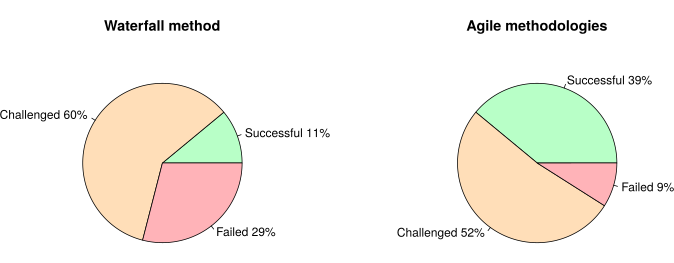
\includegraphics[width=\textwidth]{assets/charts/agile-success-rate.pdf}
	\caption{Success rate of Agile methodologies \cite{standish2015chaos}.}
	\label{fig:agile-success-rate}
\end{figure}